\section{Generalizing the \lstinline|put| and \lstinline|get| operations} \label{s:lvars-generalizing}

The determinism result for $\lambdaLVar$ shows that adding a store of
LVars to a deterministic language substrate preserves determinism.
But, even though LVars are more general than IVars, it is not the case
that the LVar @put@/@get@ interface I've described is \emph{the most
  general} interface that preserves determinism.  In this section, I
consider some alternative semantics for @put@ and @get@ that
generalize their behavior while retaining the determinism of the
original semantics.

\subsection{Generalizing from least-upper-bound writes to inflationary, commutative writes}

\lk{This will be about generalized inflationary+commutative writes,
  rather than least-upper-bound writes (lub is a special case of
  this).}

\TODO{Say something about how the lattice in
  Figure~\ref{f:lvars-example-lattices}(c) has different semantics if
  we have least-upper-bound writes or incremental writes, and how
  incremental writes may in fact be what is desired.  Possibly cite
  the CRDTs work and forward-reference Chapter~\ref{ch:distributed}.}

\lk{Here I can probably reuse some material from the PLDI and DISC
  papers and from my thesis proposal.}

\subsection{A more general formulation of threshold sets}

\begin{figure}
\begin{center}
  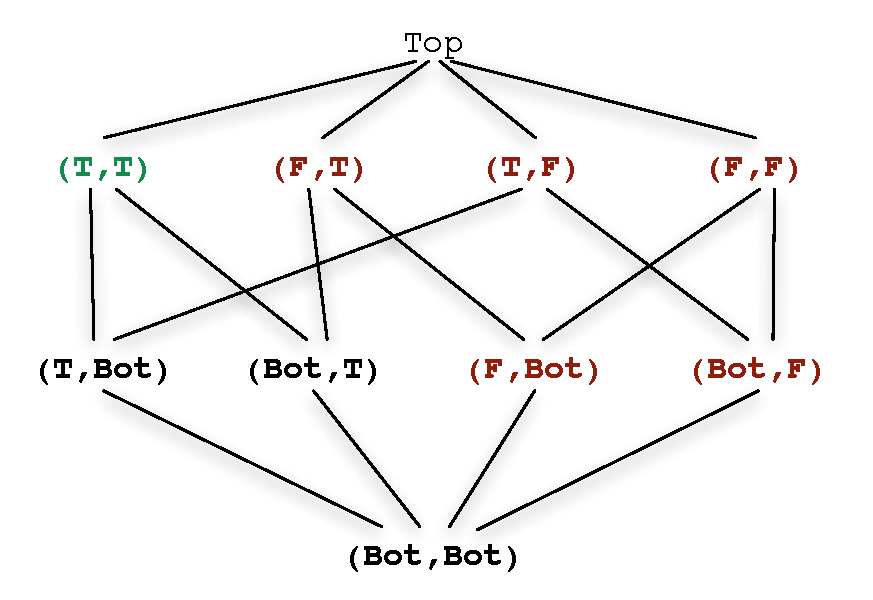
\includegraphics[width=3in]{chapter2/figures/lvars-parallel-and.pdf}
\end{center}
  \caption{Lattice of states that an \il{AndLV} can take on.  The five
    red states in the lattice correspond to a false result, and the
    one green state corresponds to a true one.}
  \label{f:lvars-parallel-and}
\end{figure}

In this section, I'll give an example of a deterministic program that
is difficult to express under our existing definition of threshold
sets, and I'll present a way to generalize our existing definition of
threshold sets to accommodate such a program.

Consider an LVar that stores the result of a parallel logical ``and''
operation on two Boolean inputs, which we'll call the \emph{left} and
\emph{right} inputs, respectively.  For convenience, we will call this
data structure an \emph{\il{AndLV}}.

We can represent the states an \il{AndLV} can take on as pairs
\il{(x,y)}, where each of \il{x} and \il{y} are \il{T}, \il{F}, or
\il{Bot}.  The \il{(Bot,Bot)} state is the state in which no input has
yet been received, and so it is the least element of the lattice of
states that our \il{AndLV} can take on, shown in
Figure~\ref{f:lvars-parallel-and}.  An additional state, \il{Top}, is
the greatest element of the lattice; it represents the situation in
which an error has occurred---if, for instance, one of the inputs
writes \il{T} and then later changes its mind to \il{F}.

The result of the parallel ``and'' computation---if it completes
successfully---will be either ``true'' or ``false'', but the
computation could also block indefinitely if not enough writes occur
(say, if the left input is \il{(T,Bot)} and the right input never
arrives), or it could terminate in an error state.

The lattice induces a lub operation on pairs of states; for instance,
the lub of \il{(T,Bot)} and \il{(Bot,F)} is \il{(T,F)}, and the lub of
\il{(T,Bot)} and \il{(F,Bot)} is \il{Top} since the overlapping \il{T}
and \il{F} values conflict.  As usual for LVars, the @put@ operation
updates the \il{AndLV}'s state to the lub of the incoming state and
the current state.

Let's consider what observations it is possible to make of an
\il{AndLV} under our existing definition of threshold reads.  The
states \il{(T,T)}, \il{(T,F)}, \il{(F,T)}, and \il{(F,F)} are all
pairwise incompatible with one another, and so $\setof{\textrm{
    \il{(T,T)}, \il{(T,F)}, \il{(F,T)}, \il{(F,F)} }}$ is a legal
threshold set argument to @get@.  The trouble with this threshold read
is that it does not allow us to get \emph{early answers} from the
computation.  It would be preferable to have a @get@ operation that
would ``short circuit'' and unblock immediately if a single input of,
say, \il{(F,Bot)} or \il{(Bot,F)} was written, since no later write
could change the fact that the result of the whole computation would
be ``false''.\footnote{Actually, this is not quite true: a write of
  \il{(F,Bot)} followed by a write of \il{(T,Bot)} would lead to a
  result of \il{Top}, and to the program stepping to the $\error$
  state, which is certainly different from a result of ``false''.
  But, even if a write of \il{(T,Bot)} is due to come along sooner or
  later to take the state of the \il{AndLV} to \il{Top} and thus raise
  $\error$, it should still be fine for the \il{get} operation to
  allow ``short-circuit'' unblocking, because the result of the
  \il{get} operation does not count as observable under our definition
  of observable determinism (as discussed in
  Section~\ref{subsection:lvars-errors-and-observable-determinism}).}
Unfortunately, we cannot include \il{(F,Bot)} or \il{(Bot,F)} in our
threshold set, because the resulting threshold set would no longer be
pairwise incompatible, and therefore would compromise determinism.

Fortunately, there \emph{is} a way to get short-circuiting behavior
from an \il{AndLV} without compromising determinism, although it will
require a slight change to how threshold sets and threshold reads
work.  In the new formulation, we divide up threshold sets into
subsets that we call \emph{activation sets}, each consisting of
\emph{activation states}.  In the case of the observation we want to
make of nour \il{AndLV}, one of those activation sets is the set of
states that the data structure might be in when a state containing at
least one \il{F} value has been written---that is, the set $\setof{
  \textrm{\il{(F,Bot)}, \il{(Bot,F)}, \il{(F,T)}, \il{(T,F)},
    \il{(F,F)}} }$.  When we reach a point in the lattice that is at
or above any of those states, we know that the result will be
``false''.  The other activation set is the singleton set $\{
\textrm{\il{(T,T)}} \}$.  When we reach the state \il{(T,T)}, we know
that the result is ``true'', but we have to wait until then; a state
like \il{(T,Bot)} doesn't appear in any of our activation sets.

We can now redefine ``threshold set'' to mean \emph{a set of
  activation sets}.  Therefore the entire threshold set for observing
the contents of our \il{AndLV} is:
\[
\{ 
\{ \textrm{\il{(F,Bot)}, \il{(Bot,F)}, \il{(F,T)}, \il{(T,F)}, \il{(F,F)}} \},
\{ \textrm{\il{(T,T)}} \}
\}
\]
And we redefine the semantics ofa a threshold read as follows: if an
LVar's state reaches (or surpasses) any state or states in a
particular set of activation states, the threshold read returns
\emph{the entire set} of activation states, regardless of which of
those activation states was reached. If no state in any set of
activation states has yet been reached, the threshold read will block.
In the case of our \il{AndLV}, as soon as either input writes a state
containing an \il{F}, our @get@ will unblock and return the first set
of activation states, that is, $\{ \textrm{\il{(F,Bot)}, \il{(Bot,F)},
  \il{(F,T)}, \il{(T,F)}, \il{(F,F)}} \}$.  Hence \il{AndLV} has the
expected ``short-circuit'' behavior and does not have to wait for a
second input if the first input contains an \il{F}.  If, on the other
hand, the inputs are \il{(T,Bot)} and \il{(Bot,T)}, the @get@ will
unblock and return $\{ \textrm{\il{(T,T)}} \}$.

In a real implementation, of course, the value returned from the @get@
could be more meaningful to the client---for instance, a Haskell
implementation could return \il{False} instead of returning the set of
activation states that corresponds to ``false''.  However, the
translation from $\{ \textrm{\il{(F,Bot)}, \il{(Bot,F)}, \il{(F,T)},
  \il{(T,F)}, \il{(F,F)}} \}$ to \il{False} could just as easily take
place on the client side.  In either case, the result returned from
the threshold read is the same regardless of \emph{which} of the
activation states caused it to unblock, and it is impossible for the
client to tell whether the actual state of the lattice is, say,
\il{(T,F)} or \il{(F,F)} or some other state containing \il{F}.

\TODO{Revise the rest of this subsection---it's dumped in from the
  DISC paper and can be made a lot shorter.}

In order for the behavior of a threshold query
to be deterministic, it must be unblocked by
a \emph{unique} set of activation states in the threshold set.  
We ensure this by
requiring that elements in a set of activation states must be
\emph{pairwise incompatible} with elements in every other set of
activation states.  That is, for all distinct sets of activation states $Q$
and $R$ in a given threshold set: $\forall q \in Q.~\forall r \in R.~q \sqcup r = \top$.
\lk{changed to inline math to save space.}
%% %
%% \[ \forall q \in Q.~\forall r \in R.~q \sqcup r = \top \]
%% %
In our \il{AndLV} example, there are two distinct sets of activation states, so if
we let $Q = \{ \textrm{\il{(T,T)}} \}$ and $R = \{
\textrm{\il{(F,Bot)}, \il{(Bot,F)}, \il{(F,T)}, \il{(T,F)},
  \il{(F,F)}} \}$, the least upper bound of \il{(T,T)} and $r$ must be
\il{Top}, where $r$ is any element of $R$.  We can easily verify that
this is the case.  Furthermore, since the lattice of states that an
\il{AndLV} can take on is finite, the join function can be verified to compute a
least upper bound.

Why is pairwise incompatibility necessary?  Consider the following
(illegal) ``threshold set'' that does not meet the pairwise
incompatibility criterion:
$ \{ \{ \textrm{\il{(F,Bot)}, \il{(Bot,F)}} \},  \{ \textrm{\il{(T,Bot)}, \il{(Bot,T)}} \} \} $.
\lk{changed to inline math to save space.}
%% \[
%% \{ 
%% \{ \textrm{\il{(F,Bot)}, \il{(Bot,F)}} \},
%% \{ \textrm{\il{(T,Bot)}, \il{(Bot,T)}} \}
%% \}
%% \]
A threshold query corresponding to this so-called threshold set will
unblock and return $\{ \textrm{\il{(F,Bot)}, \il{(Bot,F)}} \}$
as soon as a state containing an
\il{F} is reached, and $\{ \textrm{\il{(T,Bot)}, \il{(Bot,T)}} \}$
as soon as a state
containing a \il{T} is reached.  The trouble with such a threshold
query is that there exist states, such as \il{(F,T)} and \il{(T,F)},
that could unblock either set of activation states.  If the left input
writes \il{F} and the right input writes \il{T}, and these writes
occur in arbitrary order, then the threshold query will return a
nondeterministic result, depending on the order in which the two
writes arrive.  But with the original, pairwise-incompatible threshold
set we showed, the threshold query would deterministically return
\il{False}---although if the \il{T} arrived first, the query would
have to block until the \il{F} arrived, whereas if the \il{F} arrived
first, it could unblock immediately.  Hence threshold queries enforce
consistency at the expense of availability, but it is still possible
to do a ``short-circuit'' computation that unblocks as soon as an
\il{F} is written.

The threshold set mechanism we describe in this section is 
part of the LVars programming model discussed in
section~\ref{s:intro}; in fact, our \il{AndLV} example is precisely an
LVar~\cite{effectzoo}.  But the utility of threshold queries
is not limited to LVars.  In
the following sections, we review the basics of the CvRDT model from the work of
Shapiro \etal, then show how to add threshold queries to the CvRDT
model, and prove that they are strongly
consistent queries.

\subsection{Generalizing from threshold sets to threshold functions}


\TODO{Write this subsection!}

\lk{This will be about "threshold functions", rather than either
  simple threshold sets or generalized threshold sets (i.e., partial
  functions that take a lattice element and are undefined for all
  inputs that are not at or above a given point in the lattice, and
  constant for all inputs that are at or above that point; both kinds
  of threshold sets are a special case of this, afaict).}
